
\section{Force and Motion I\footnote{
1990-93 Dept. of Physics and Astronomy, Dickinson College. Supported by FIPSE
(U.S. Dept. of Ed.) and NSF. Portions of this material may have been modified
locally and may not have been classroom tested at Dickinson College.
}}

\makelabheader %(Space for student name, etc., defined in master.tex or labmanual_formatting_commands.tex)

\textbf{Objectives }

\begin{itemize}
\item To learn how to use a force probe to measure force. 
\item To understand the relationship between forces applied to an object and its motions. 
\item To find a mathematical relationship between the force applied to an object and its acceleration.
\end{itemize}
\textbf{Overview }

In the previous labs, you have used a motion detector to display position-time,
velocity-time and acceleration-time graphs of the motion of different objects.
You were not concerned about how you got the objects to move, i.e., what forces
(pushes or pulls) acted on the objects. From your experiences, you know that
force and motion are related in some way. To start your bicycle moving, you
must apply a force to the pedal. To start up your car, you must step on the
gas pedal to get the engine to apply a force to the road through the tires.

But, exactly how is force related to the quantities you used in the previous
unit to describe motion --- position, velocity and acceleration? In this unit you
will pay attention to forces and how they affect motion. You will apply forces
to a cart, and observe the nature of its resulting motion graphically with a
motion detector.

\textbf{Apparatus} 

\begin{itemize}
\item Force probe 
\item Variety of hanging masses 
\item CS2000 compact scale (for measuring mass)
\item Low friction pulley and string 
\item Motion detector 
\item Dynamics cart and track 
\item \textit{Science Workshop 750 Interface}
\item \textit{Capstone} software (V, A \& F Graphs application)
\end{itemize}
\textbf{Measuring Forces} 

In this investigation you will use a force probe (also called a force sensor) to measure forces. The force probe puts out a voltage signal proportional to the force applied to the arm of the probe. Physicists have defined a standard unit of force called the newton, abbreviated N. For your work on forces and the motions they cause, it will be more convenient to have the force probe read directly in newtons rather than voltage. Before the force probe is used it must be calibrated. Before calibrating the force probe, open the \textbf{V, A \& F Graphs 750.cap} application in the \textbf{131 Capstone 750} folder. To calibrate the force probe, see \textit{Calibrating Force Sensors} in \textbf{Appendix \ref{capstone}: Capstone}.

\pagebreak[2]
\textbf{Motion and Force} 

Now you can use the force probe to apply measured amounts of force to an object.
You can also use the motion detector, as in the previous units, to examine the
motion of the object. In this way you will be able to establish the relationship
between motion and force.
\vspace{10mm}

\textbf{Activity 1: Pushing and Pulling a Cart} 

In this activity you will move a cart by pushing and pulling it with your hand.
You will measure the force, velocity and acceleration. Then you will be able
to look for relationships between the applied force and the motion quantities,
to see which is (are) related to force.

(a) Calibrate the force probe if you haven't already done so (see \textit{Calibrating Force Sensors} in \textbf{Appendix \ref{capstone}: Capstone}). Then set up the cart, force probe and motion detector on the level track as shown in Figure 1. Measure the mass of the cart and force probe assembly (using the compact scale). Record the result here:

\answerspace{15mm}

\begin{figure}[t]
{\par\centering 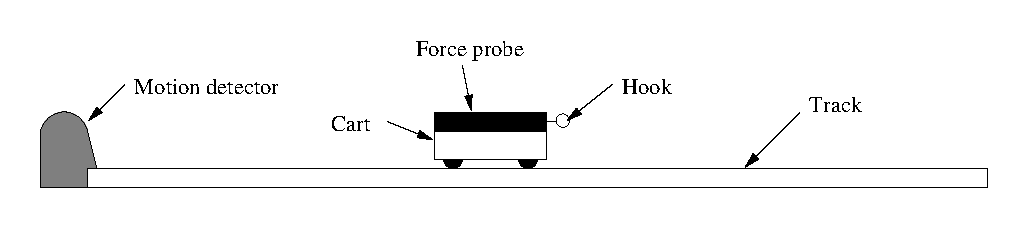
\includegraphics{force1/force1_fig1.eps} \par}


\caption{Equipment setup for qualitative measurements of force and motion.}
\end{figure}


(b) Suppose you grasp the hook on the force probe and move the cart forwards
and backwards in front of the motion detector. Do you think that either the
velocity or the acceleration graph will look like the force graph? Is either
of these motion quantities related to force? That is to say, if you apply a
changing force to the cart, will the velocity or acceleration change in the
same way as the force?
\answerspace{35mm}

\pagebreak[3]
(c) To test your predictions, click the \textbf{Record} button, grasp the
hook on the force probe and push and pull the cart back and forth 3 or 4 times. Be sure that
the cart never gets closer than 0.15 m away from the detector and be careful
of the wires. Repeat until you get a good run, and adjust the sampling time
and scale of the axes if necessary. Sketch your graphs on the axes that follow.

\vspace{0.3cm}
{\par\centering 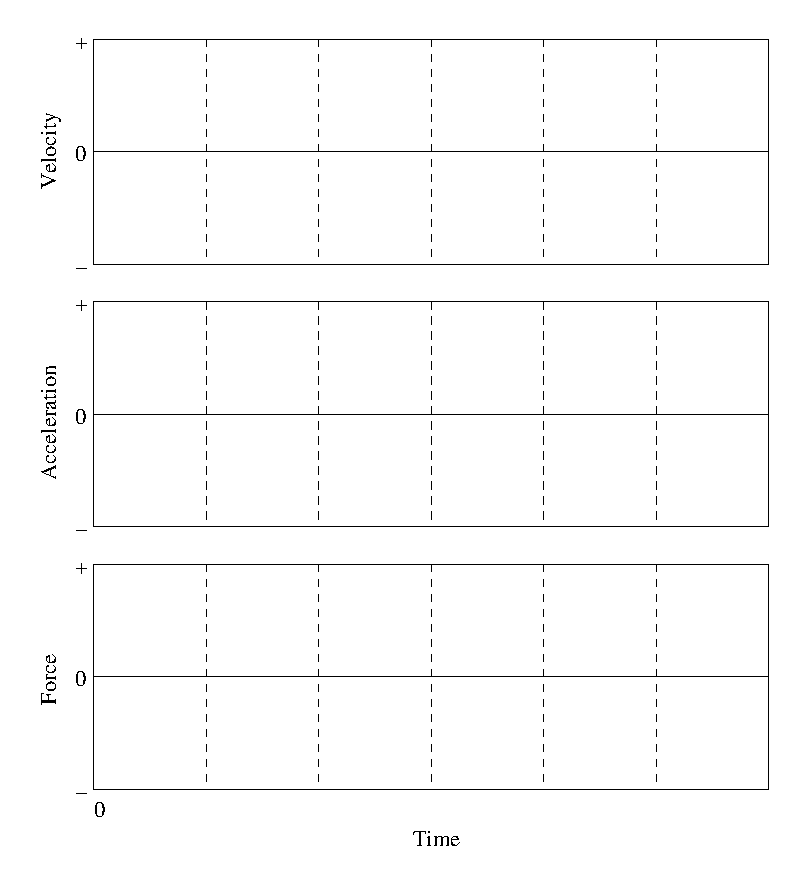
\includegraphics{force1/force1_fig2.eps} \par}
\vspace{0.3cm}

(d) Does either graph--velocity or acceleration--resemble the force graph? Which
one? Explain.
\answerspace{20mm}

(e) Based on your observations, does it appear that either the velocity or acceleration
of the cart might be related to the applied force? Explain.
\answerspace{20mm}

\pagebreak[3]
\textbf{Activity 2: Speeding Up }

You have seen in the previous activity that force and acceleration seem to be
related. But just what is the relationship between force and acceleration? 

(a) Suppose you have a cart with very little friction, and that you pull this
cart with a constant force as shown below on the force-time graph. Predict with sketches on
the axes below the velocity-time and acceleration-time graphs of the cart's motion.

\vspace{0.3cm}
{\par\centering 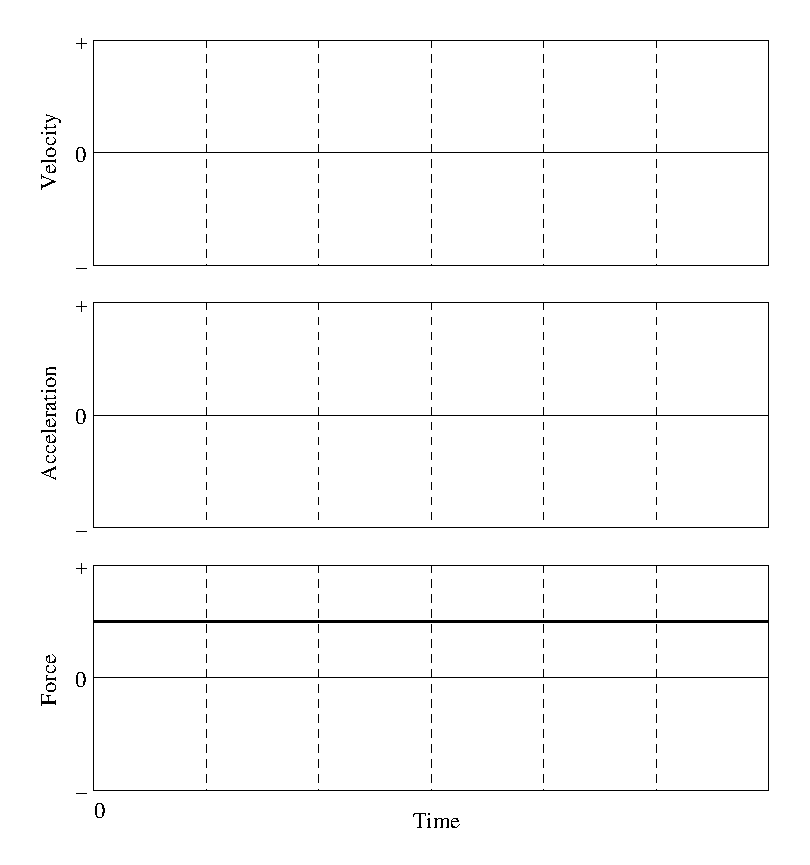
\includegraphics{force1/force1_fig3.eps} \par}
\vspace{0.3cm}

(b) Describe in words the predicted shape of the velocity \textit{vs.}~time and acceleration
vs. time graphs for the cart.
\vspace{20mm}

\newpage

(c) Test your predictions. Set up the pulley, cart, string, motion detector
and force probe as shown in Figure 2. The cart should be the same mass as before. Hang 50 g from the end of the string. Start the data acquisition.
Release the cart when you hear the clicks of the motion detector. Be sure that
there is enough slack in the force probe cables to complete the motion and catch
the cart before it crashes into the pulley. Repeat until you get good graphs
in which the cart is seen by the motion detector over the entire motion. Sketch
the actual velocity, acceleration and force graphs for the motion of interest
on the axes below and indicate the scale on the axes. Draw smooth graphs; don't
worry about small bumps.

\begin{figure}
{\par\centering 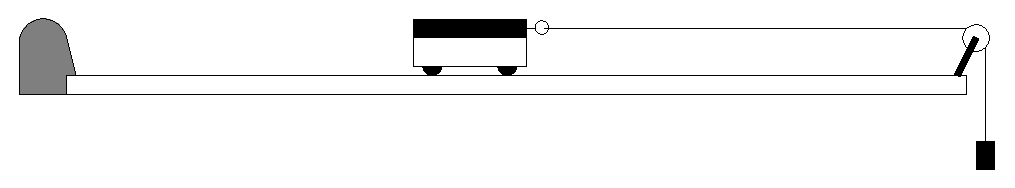
\includegraphics{force1/force1_fig4.eps} \par}


\caption{Equipment setup for quantitative measurements of force and motion.}
\end{figure}


\vspace{0.3cm}
{\par\centering 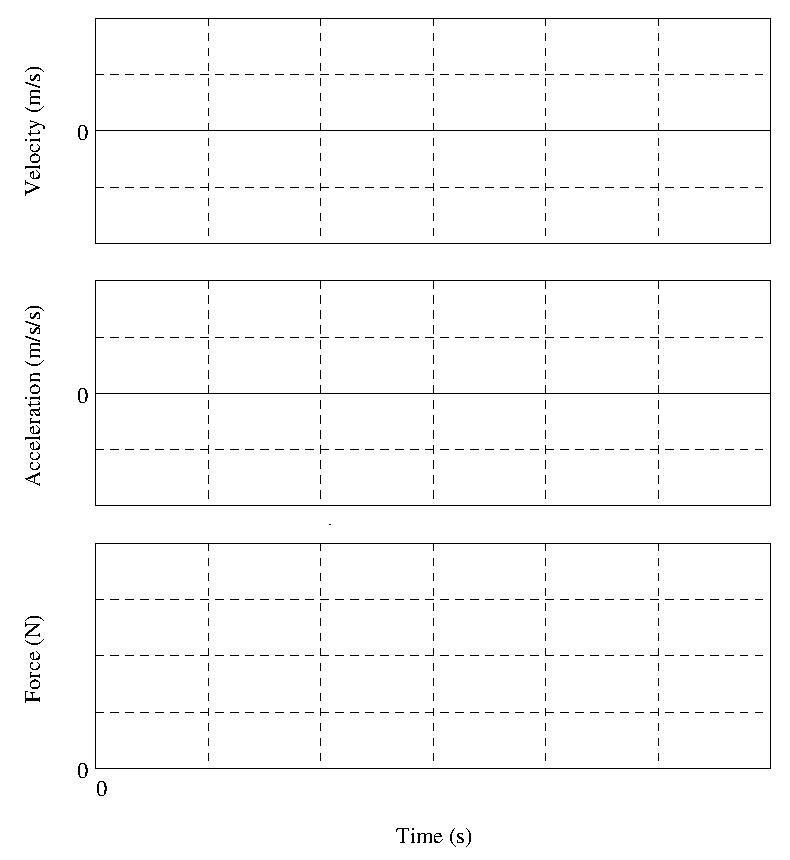
\includegraphics[width=0.65\textwidth]{force1/force1_fig5.eps} \par}
\vspace{0.3cm}

(d) Is the force which is applied to the cart by the string constant, increasing
or decreasing? Explain based on your graph.
\answerspace{15mm}

\pagebreak[2]
(e) How does the acceleration graph vary in time? Does this agree with your
prediction? What kind of acceleration corresponds to a constant applied force?
\answerspace{20mm}

(f) How does the velocity graph vary in time? Does this agree with your prediction?
What kind of velocity corresponds to a constant applied force?
\answerspace{20mm}

(g) Use the \textbf{Statistics} function to determine the average force and the average acceleration
and record them below. Find the mean values only during the time interval when
the force and acceleration are nearly constant. See \textbf{Appendix \ref{capstone}} for details on
the use of the \textbf{Statistics} function of Capstone.
\answerspace{20mm}

\textbf{Activity 3: Acceleration from Different Forces }

In the previous activity you have examined the motion of a cart with a constant
force applied to it. But, what is the relationship between acceleration and
force? If you apply a larger force to the same cart (same mass as before) how
will the acceleration change? In this activity you will try to answer these
questions by applying a different force to the cart, and measuring the corresponding
acceleration. 

(a) Suppose you pulled the cart with a force about twice as large as before.
What would happen to the acceleration of the cart? Explain.
\answerspace{20mm}

\pagebreak[3]
(b) Test your prediction by replacing the 50-g mass with a 100-g mass and creating graphs of the motion as before. Repeat until you have a good run. Sketch the
results on the axes that follow. Don't forget to put the scale on the axes.

\vspace{0.3cm}
{\par\centering 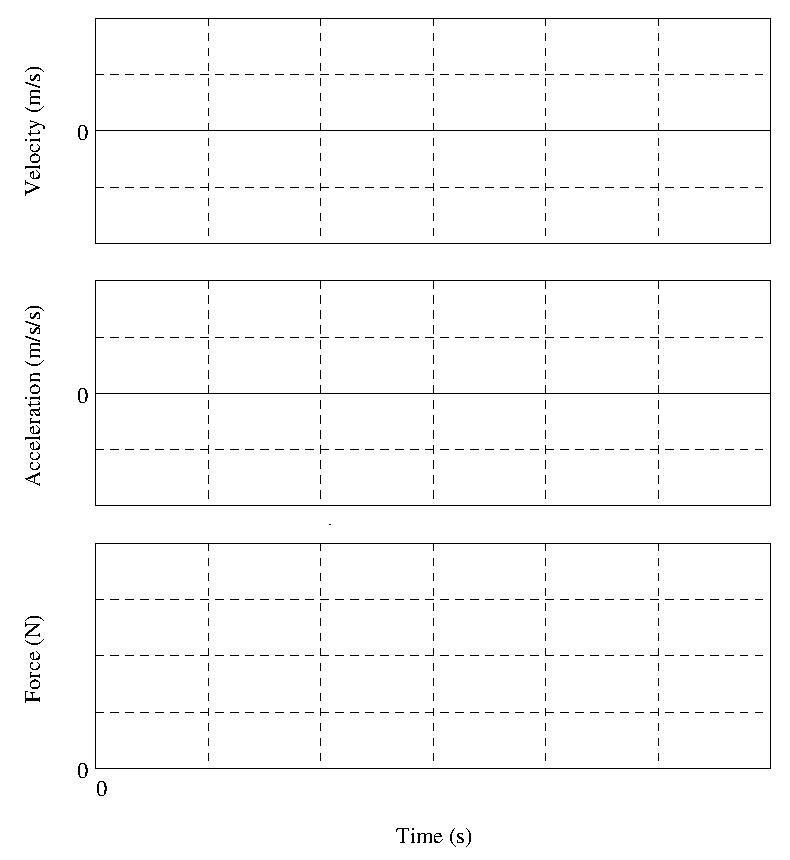
\includegraphics[width=0.65\textwidth]{force1/force1_fig5.eps} \par}
\vspace{0.3cm}

(c) Use the \textbf{Statistics} function to find the average force and the average acceleration
and record them below. Find the mean values only during the time interval when
the force and acceleration are nearly constant.
\answerspace{15mm}

(d) How did the force applied to the cart compare to that with the smaller force
in Activity 2?
\answerspace{15mm}

(e) How did the acceleration of the cart compare to that caused by the smaller
force in Activity 2? Did this agree with your prediction? Explain.
\answerspace{15mm}

\pagebreak[2]
\textbf{Activity 4: The Relationship Between Acceleration and Force }

If you accelerate the same cart (same mass) with another force, you will then
have three data points--enough data to plot a graph of acceleration \textit{vs.}~force.
You can then find the mathematical relationship between acceleration and force. 

(a) Accelerate the cart with a force roughly midway between the other two forces
tried. Use a hanging mass about midway between those used in the last two activities.
Record the mass below.
\answerspace{10mm}

(b) Graph velocity, acceleration and force. Sketch the graphs on the axes in
Activity 3 using dashed lines.

(c) Find the mean acceleration and force, as before, and record the values in
the table below (in the Activity 4 line). Also, enter the values from the previous two activities in the table.

\vspace{0.3cm}
{\centering \begin{tabular}{|c|c|c|}
\hline 
&
Average Force (N)&
Average Acceleration (m/s\( ^{2} \))\\
\hline 
Activity 2&
&
\\
&
&
\\
\hline 
Activity 4&
&
\\
&
&
\\
\hline 
Activity 3&
&
\\
&
&
\\
\hline 
\end{tabular}\par}
\vspace{0.3cm}

(d) Using \textit{Excel}, plot the average force applied to the cart as a function of the average acceleration of the cart by fitting the data with a linear function. Include a fourth data point (0,0) (since zero force means 0 acceleration). Label and print the graph showing the best fit, and add it to this unit.

(e) Does there appear to be a simple mathematical relationship between the acceleration of a cart (with fixed mass) and the force applied to the cart (measured by the force probe mounted on the cart)? Write down the equation you found and describe the mathematical relationship in words.  What is the slope of the graph?
\answerspace{20mm}

(f) Use the LINEST function in \textit{Excel} (see \textbf{Appendix \ref{excel}: Excel}) to determine the uncertainty in mass of the cart/force sensor combination based on your data points.  Write your result as \textit{Mass} = $m$ \( \pm \ \Delta  m\). Be sure and include proper units.
\answerspace{20mm}

(g) Does your measurement of $m$ from Activity 1 fall within the range indicated in (f) above? If not, what are some possible sources of systematic error?
\answerspace{20mm}

Comment: The relationship which you have been examining between the acceleration of the cart and the applied force is known as Newton's Second Law, \textit{F = ma.}

\pagebreak[2]
\textbf{Homework} 

1. A force is applied which makes an object move with the acceleration shown
below. Assuming that friction is negligible, sketch a force-time graph of the
force on the object on the axes below.

\vspace{0.3cm}
{\par\centering 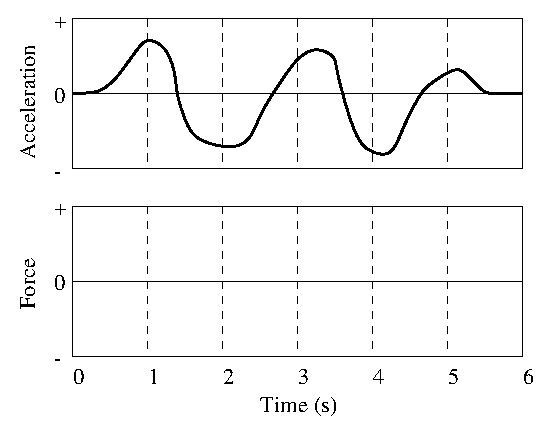
\includegraphics{force1/force1_fig6.eps} \par}
\vspace{0.3cm}

Explain your answer:
\vspace{10mm}

2. Roughly sketch the velocity-time graph for the object in question 1 on the
axes below, beginning with a \textit{negative} velocity.  Remember that acceleration 
is the 
\ifForOneTwentyFive
   \textit{slope} 
\else
   \textit{derivative} 
\fi
of velocity.

\vspace{0.3cm}
{\par\centering 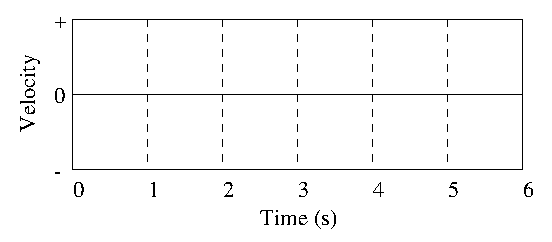
\includegraphics{force1/force1_fig7.eps} \par}
\vspace{0.3cm}

3. A cart can move along a horizontal line (the + position axis). It moves with
the velocity shown below.

\vspace{0.3cm}
{\par\centering 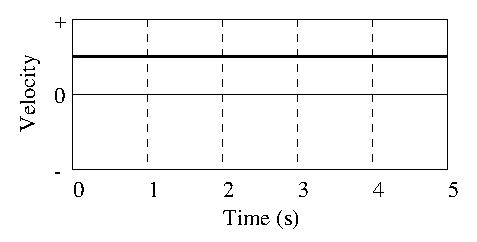
\includegraphics{force1/force1_fig8.eps} \par}
\vspace{0.3cm}

\pagebreak[2]
Assuming that friction is so small that it can be neglected, sketch on the axes
that follow the acceleration-time and force-time graphs of the cart's motion.

\vspace{0.3cm}
{\par\centering 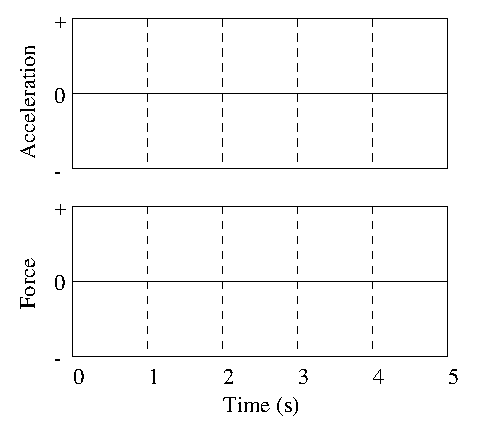
\includegraphics{force1/force1_fig9.eps} \par}
\vspace{0.3cm}

Explain both of your graphs.
\answerspace{20mm}

Questions 4-6 refer to an object which can move in either direction along a
horizontal line (the + position axis). Assume that friction is so small that
it can be neglected. Sketch the shape of the graph of the force applied to the
object which would produce the motion described. 

4. The object moves away from the origin with a constant acceleration.

\vspace{0.3cm}
{\par\centering 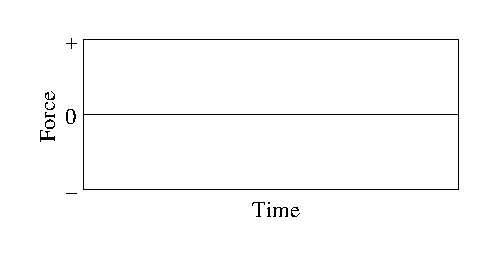
\includegraphics[scale=1.1]{force1/force1_fig10.eps} \par}
\vspace{0.3cm}

5. The object moves toward the origin with a constant acceleration.

\vspace{0.3cm}
{\par\centering 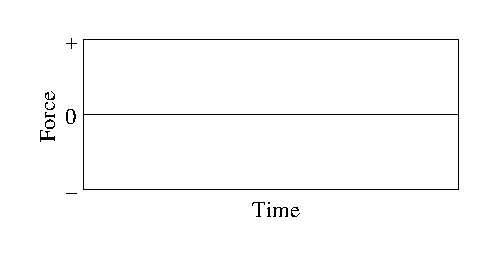
\includegraphics[scale=1.1]{force1/force1_fig10.eps} \par}
\vspace{0.3cm}

\pagebreak[2]
6. The object moves away from the origin with a constant velocity.

\vspace{0.3cm}
{\par\centering 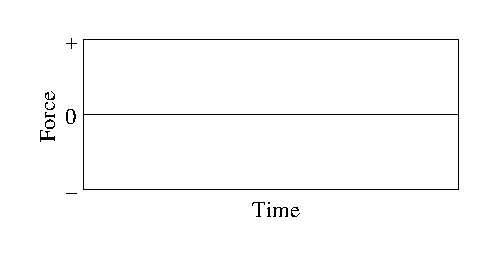
\includegraphics[scale=1.1]{force1/force1_fig10.eps} \par}
\answerspace{0.3cm}

Questions 7 and 8 refer to an object which can move along a horizontal line
(the + position axis). Assume that friction is so small that it can be ignored.
The object's velocity-time graph is shown below.

\vspace{0.3cm}
{\par\centering 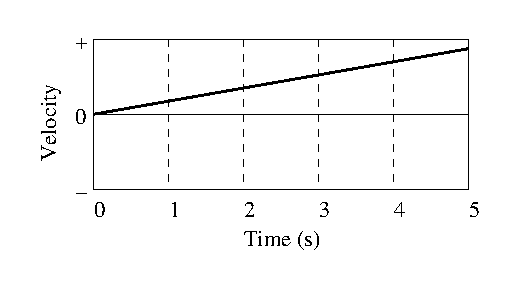
\includegraphics[scale=1.1]{force1/force1_fig11.eps} \par}
\answerspace{0.3cm}

7. Sketch the shapes of the acceleration-time and force-time graphs on the axes
below.

\vspace{0.3cm}
{\par\centering 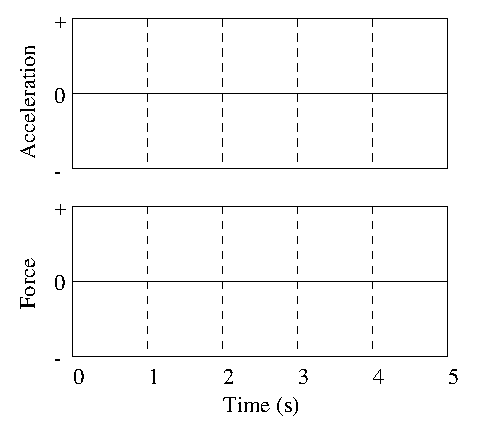
\includegraphics[scale=1.1]{force1/force1_fig9.eps} \par}
\answerspace{0.3cm}

8. Suppose that the force applied to the object were twice as large. Sketch
with dashed lines on the same axes above the force, acceleration, and velocity.

\pagebreak[4]
Question 9 refers to an object which can move along a horizontal line (the +
position axis). Assume that friction is so small that it can be ignored. The
object's velocity-time graph is shown below.

\vspace{0.3cm}
{\par\centering 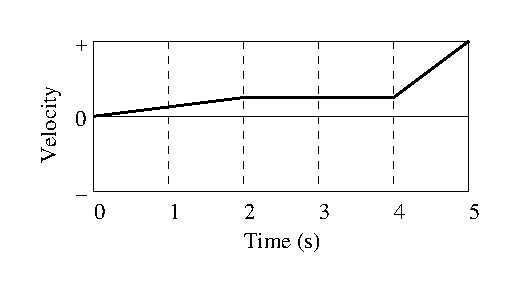
\includegraphics{force1/force1_fig12.eps} \par}
\vspace{0.3cm}

9. Sketch the shapes of the acceleration and force graphs on the axes below.

\vspace{0.3cm}
{\par\centering 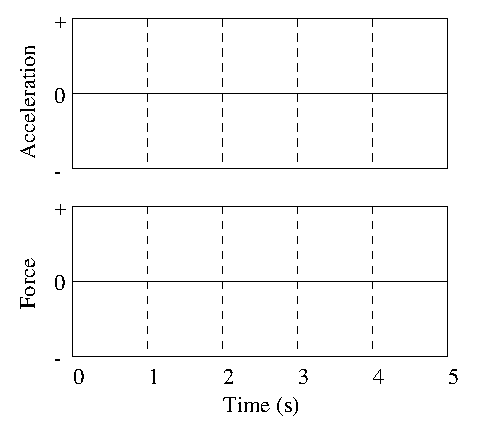
\includegraphics{force1/force1_fig9.eps} \par}
\vspace{0.3cm}

